\subsection{Háttér}

%21
\begin{frame}
  HTML elemek hátterével kapcsolatos tulajdonságok:
  \begin{description}[m]
    \item[\texttt{background-color}] \hfill \\ A háttér színe. 
    Alapértelmezetten \texttt{transparent}, azaz átlátszó.
    \item[\texttt{background-image}] \hfill \\ Háttérkép, amivel 
    alapértelmezés szerint kicsempézi az elem teljes területét 
    (margókat nem). 
    Alapértéke \texttt{none}, nincs háttérkép. Az \texttt{url()} 
    függvény paramétereként adható meg a képfájl, pl. \\
    \texttt{background-image: url("hatter.png");} \\Megadhatók 
    \hiv{\href{https://cssgradient.io/}{színátmenetek}} is.\\
    A szöveg maradjon \kiemel{olvasható} a háttéren!
  \end{description}
\end{frame}

%22
\begin{frame}
  \begin{description}[m]
    \item[\texttt{background-repeat}] \hfill \\ Háttérkép 
    csempézési iránya
    \begin{itemize}
      \item \texttt{repeat} mindkét irányban, túlnyúló részek 
      levágásával, alapértelmezés
      \item \texttt{repeat-x} csak vízszintesen
      \item \texttt{repeat-y} csak függőlegesen
      \item \texttt{no-repeat} csak egyszer, alapértelmezetten a bal 
      felső sarokban
      \item \texttt{round} torzítja a képet a vágás elkerülésére
      \item \texttt{space} csak annyiszor ismétel, ami vágás 
      nélkül elfér, közöttük helyet hagy
    \end{itemize}
    Két érték megadásakor az első a vízszintes, második a 
    függőleges irányra vonatkozik.
  \end{description}
\end{frame}

%23
\begin{frame}
  \begin{center}
    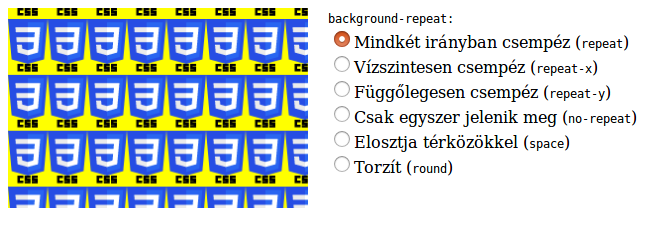
\includegraphics[width=.75\textwidth]{hatter.png}\\
    \textattachfile{hatter.html}{hatter.html}, \textattachfile{css3.svg}{css3.svg}
  \end{center}
\end{frame}

%24
\begin{frame}
  \begin{description}[m]
    \item[\texttt{background-position}] \hfill \\ Igazítás, a 
      \emph{vízszintes} és a \emph{függőleges} pozíciót várja. Ha egyet 
      kap, a másik \texttt{center} lesz.
      \begin{itemize}
        \item Függőlegesen: \texttt{left}, \texttt{center}, 
        \texttt{right}
        \item Vízszintesen: \texttt{top}, \texttt{center}, 
        \texttt{bottom}
        \item Mindkettőnél lehet százelékot, vagy egyéb CSS 
        mértékegységet (pl. képpont) használni. 
      \end{itemize}
  \end{description}
\end{frame}

%25
\begin{frame}
  \begin{exampleblock}{\textattachfile{pozicio1.html}{pozicio1.html}}
    \fontsize{7}{8} \selectfont
    \lstinputlisting[style=HTML,linerange={7-11},numbers=left,firstnumber=7]{pozicio1.html}
    \lstinputlisting[style=HTML,linerange={15-16},numbers=left,firstnumber=15]{pozicio1.html}
    \lstinputlisting[style=HTML,linerange={24-25},numbers=left,firstnumber=24]{pozicio1.html}
    \lstinputlisting[style=HTML,linerange={37-38},numbers=left,firstnumber=37]{pozicio1.html}
    \lstinputlisting[style=HTML,linerange={53-54},numbers=left,firstnumber=53]{pozicio1.html}
  \end{exampleblock}
\end{frame}

%26
\begin{frame}
  \begin{description}[m]
    \item[\texttt{background-attachment}] \hfill \\
      \begin{itemize}
        \item \texttt{scroll} a háttér együtt gördül az oldallal, 
        alapértelmezés
        \item \texttt{fixed} rögzített háttér
        \item \texttt{local} az elem tartalmával együtt gördül a háttér
      \end{itemize}
      \vfill
      A logo mindig a jobb alsó sarokban: 
      \textattachfile{rogzites1.html}{rogzites1.html}\\
      Két bekezdés között kilátszik a háttérben rögzített logo: 
      \textattachfile{rogzites2.html}{rogzites2.html}
  \end{description}
\end{frame}

%27
\begin{frame}
  \begin{description}[m]
    \item[\texttt{background}] \hfill \\ Rövidítés: egy összetett 
    tulajdonsággal sok egyszerű tulajdonság értéke állítható 
    be. \kiemel{Értékek sorrendje rögzített, de tetszőleges 
    számú érték elhagyható!}\\
    \texttt{background: \emph{background-color background-image 
    background-repeat}\\
    \qquad\emph{background-attachment background-position}}
  \end{description}
  \begin{columns}[T]
    \column{0.5\textwidth}
      \begin{exampleblock}{\textattachfile{pozicio1.html}{pozicio1.html}}
        \fontsize{7}{8} \selectfont
        \lstinputlisting[xleftmargin=-1cm,style=HTML,linerange={7-11}]{pozicio1.html}
      \end{exampleblock}
    \column{0.5\textwidth}
      \begin{exampleblock}{\textattachfile{pozicio2.html}{pozicio2.html}}
        \fontsize{7}{8} \selectfont
        \lstinputlisting[xleftmargin=-1cm,style=HTML,linerange={7-10}]{pozicio2.html}
      \end{exampleblock}
  \end{columns} 
\end{frame}

%28
\begin{frame}
  \begin{description}[m]
    \item[\texttt{background-size}] \hfill \\
      \begin{itemize}
        \item \texttt{auto}: Alapértelmezés, eredeti méret.
        \item \emph{szélesség, magasság}: utóbbi elhagyásával 
        \texttt{auto}-t feltételez. Használhatók CSS 
        mértékegységek és százalékok (\kiemel{a szülő elem mérete a 
        100\%}, nem a sajátja!).
        \item \texttt{cover} Addig nyújt és vág, amíg le nem fedi a 
        szülő elem teljes területét.
        \item \texttt{contain} Addig nyújt, amíg egyszer bele nem fér a 
        háttér a szülő elembe.
      \end{itemize}
  \end{description}
  \vfill
  \begin{center}
    
\includegraphics[scale=0.3]{meret.png}\\
    \textattachfile{meret.html}{meret.html}, \textattachfile{css3.svg}{css3.svg}
  \end{center}
\end{frame}

%29
\begin{frame}
  \begin{columns}[c]
    \column{0.5\textwidth}
      \footnotesize
      Induljon ki a \textattachfile{rogzites2.html}{rogzites2.html} 
      fájlból, és alakítsa át a jobb oldali ábrának megfelelően!
      \begin{itemize}
        \item Az írásszín legyen világos szürke!
        \item A teljes oldal háttere legyen kék (RGB-összetevők: 0, 
        145 és 190)!
        \item A \texttt{<div>} elem háttereként állítsa be a 
        \textattachfile{HTML5sticker.png}{HTML5sticker.png} fájl!
        \item Ennek helyzete ne függjön a görgetéstől!
        \item Helyezze el azt a képernyő közepén!
        \item A képet méretezze aránytartó módon úgy, hogy éppen 
        kitöltse a rendelkezésre álló helyet!
        \item Próbálja mindezt a lehető legkevesebb CSS tulajdonság 
        felhasználásával elérni!
      \end{itemize}
    \column{0.5\textwidth}
      \begin{exampleblock}{\textattachfile{rogzites3-mo.html}{rogzites3-mo.html}, \textattachfile{HTML5sticker.png}{HTML5sticker.png}}
        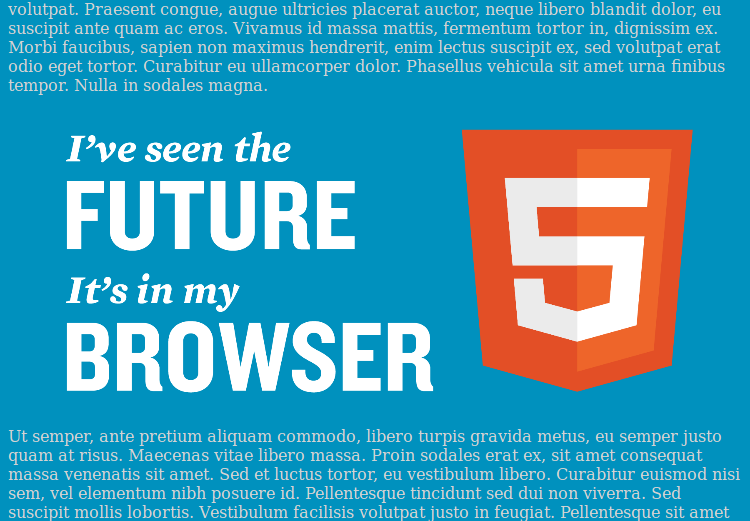
\includegraphics[width=\textwidth]{rogzites3-mo.png}
      \end{exampleblock}
  \end{columns} 
\end{frame}
